\input{../../.preambles/01-semester_work}
\input{../../.preambles/10-russian}
\input{../../.preambles/20-math}
\input{../../.preambles/22-vectors}
\input{../../.preambles/30-physics}
\usepackage{wrapfig}

\begin{document}
\maketitlepage{Факультет электроники и вычислительной техники}{физики}
{Вакуумная и газоразрядная электроника}{}{18}{студент группы Ф-369\\Голубев~А.~В.}
{}{доцент Ковтун~Д.~Г.}{}{}

\emph{Задача №1:} Электрон со скоростью \( v \) влетает в область, где 
существуют коллинеарные однородные электрическое \( E \) и магнитное \( B \) 
поля, под углом \( \alpha \) к направлению полей. Определить траекторию 
его движения и время, за которое он достигнет экрана, находящегося на 
расстоянии \( L \) от плоскости влёта, и координаты точки на экране.

\emph{Решение:}

\begin{wrapfigure}[8]{l}{0.5\textwidth}
    \vspace{-2ex}
    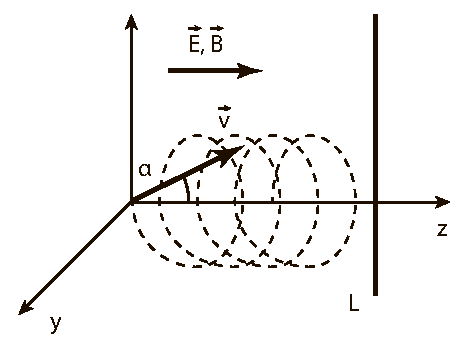
\includegraphics[width=0.5\textwidth]{images/im_01}
\end{wrapfigure}

Запишем силу действующую на электрон со стороны полей:
\[
	m\vec{a} = q\left( \vec{E} + \vec{v}\times\vec{B} \right)
\]
\[
	\vec{v}\times\vec{B} = 
	\begin{vmatrix}
		\vec{e_x} & \vec{e_y} & \vec{e_z} \\
		\dot{x}   & \dot{y}   & \dot{z}   \\
		0         & 0         & B
	\end{vmatrix}
\]

Расписывая определитель получаем систему уравнений:
\[
	\left\{ \begin{array}{ll}
		m\ddot{x} = q\dot{y}B \\
		m\ddot{y} = -q\dot{x}B \\
		m\ddot{z} = qE
	\end{array} \right.
	\quad
	\left\{ \begin{array}{ll}
		\ddot{x} = \omega_c\dot{y} \\
		\ddot{y} = -\omega_c\dot{x} \\
		\ddot{z} = \cfrac{q}{m}E
	\end{array} \right.
\]

где обозначим за \( \omega_c = \cfrac{q}{m}B \)

Найдём время за которое электрон достигнет экрана. Из уравнения 
\[ \ddot{z} = \cfrac{q}{m}E \]

Проинтегрировав уравнение по времени получим:
\[
	z = \frac{q}{2m}Et^2 + v_{z0}t
\]

Подставляя расстояние \( L \) до экрана найдём время:
\[
	L = \frac{q}{2m}Et^2 + v_{z0}t \quad\Rightarrow\quad
	\frac{q}{2m}Et^2 + v_{z0}t - L = 0
\]
\[
	t^2 + \frac{2mv_{z0}}{qE}t - \frac{2mL}{qE} = 0
\]
\[
	t = -\cfrac{mv_{z0}}{qE} + 
	\sqrt{ \cfrac{m}{qE}\left( \cfrac{mv^2_{z0}}{qE} + 2L \right)}
\]

или подставляя значение \( v_{z0} = v\cos\alpha \)
\[
	t = -\cfrac{mv_{z0}}{qE} + 
	\sqrt{ \cfrac{m}{qE}\left( \cfrac{mv^2\cos^2\alpha}{qE} + 2L \right)}
\]

Решим систему уравнений и найдём вид траектории.
\[
	\left\{ \begin{array}{ll}
		\ddot{x} = \omega_c\dot{y} \\
		\ddot{y} = -\omega_c\dot{x}
	\end{array}\right.
\]

Положим решение в виде \( \Phi = x + iy \). Домножая второе уравнение на 
мнимую единицу и складывая получим:
\[
	\ddot{\Phi} = \ddot{x} + i\ddot{y} = 
	\omega_c\dot{y} - i\omega_c\dot{x} = 
	-i\omega_c\left( \dot{x} + i\dot{y} \right) = 
	-i\omega_c\dot{\Phi}
\]

Имеем дифференциальное уравнение относительно \( \Phi \)
\[\ddot{\Phi} = -i\omega_c\dot{\Phi} \]

Решение представимо в виде:
\[
	\Phi = R_0 e^{-i\omega_c t} + C
\]

Подставляя начальные условия \( t = 0, x = y = z = 0 \), получаем значение 
константы \( C = -R_0 \). Также подставляя значения скоростей по осям 
\( x \) и \( y \) получим:
\[
	\dot{\Phi} = v_{x0} + iv_{y_0} = -R_0 i\omega_c
\]

получаем значение 
\( 
	R_0  = \cfrac{v_{x0} + iv_{y0}}{-i\omega_c} = 
	-\cfrac{v_{y0} - iv_{x0}}{\omega_c} 
\)

Подставляя полученные значения в основное уравнение, найдём вид траектории:
\[
	\Phi = -\cfrac{v_{y0} - iv_{x0}}{\omega_c} 
	\left( e^{-i\omega_c t} - 1 \right ) = 
	\left[ \cfrac{v_{y0}}{\omega_c} - i \cfrac{v_{x0}}{\omega_c} \right]
	\left( 1 - e^{-i\omega_c t} \right)
\]
\[
	\Phi = 
	\left[ \cfrac{v_{y0}}{\omega_c} - i \cfrac{v_{x0}}{\omega_c} \right]
	\cdot\Big[ 1 - \cos\left(\omega_c t\right) + 
		i\sin\left( \omega_c t\right) \Big] 
\]

Выписывая слагаемые с мнимой единицей к \( y \) и без к \( x \), получим:
\[
	\begin{array}{ll}
		x = \cfrac{v_{y0}}{\omega_c}
			\Big[ 1 - \cos\left( \omega_c t \right) \Big] + 
			\cfrac{v_{x0}}{\omega_c}\sin\left( \omega_c t \right) \\
		y = -\cfrac{v_{x0}}{\omega_c}
			\Big[ 1 - \cos\left( \omega_c t \right) \Big] + 
			\cfrac{v_{y0}}{\omega_c}\sin\left( \omega_c t \right) \\
	\end{array}
\]

Делая преобразования получим:
\[
	\left( x - \frac{v_{y0}}{\omega_c} \right)^2 + 
	\left( y + \frac{v_{yx}}{\omega_c} \right)^2 = 
	\cfrac{v^2_{x0} + v^2_{y0}}{\omega^2_c} 
	\Rightarrow R = \cfrac{v_{x0}}{\omega_c} = 
	\cfrac{v\sin\alpha}{\omega_c}
\]

\begin{wrapfigure}[10]{l}{0.5\textwidth}
    \vspace{-2ex}
    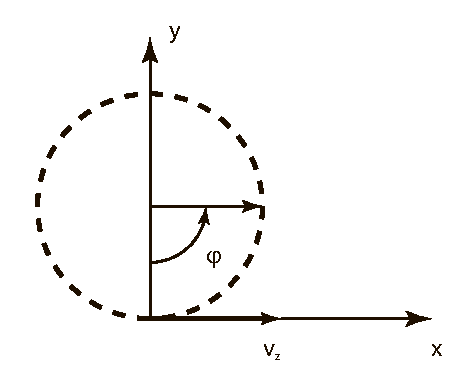
\includegraphics[width=0.5\textwidth]{images/im_02}
\end{wrapfigure}

Электрон совершает движение по окружности в плоскости \( xy \). 
В пространстве электрон перемещается по спирали.

Найдём координаты точки на экране. С учётом того \( v_{y0} = 0 \), уравнения 
движения перепишутся в виде:
\[
	\left\{ \begin{array}{ll}
		x = \cfrac{v\sin\alpha}{\omega_c}\sin\left( \omega_c t \right) \\
		y = -\cfrac{v\sin\alpha}{\omega_c}
			\Big[ 1 - \cos\left( \omega_c t \right) \Big]
	\end{array} \right.
\]

где \( t \) определяется выражением:
\(
	t = -\cfrac{mv_{z0}}{qE} + 
	\sqrt{ \cfrac{m}{qE}\left( \cfrac{mv^2\cos^2\alpha}{qE} + 2L \right)} 
\)

\pagebreak

%-------------------------------------------------------------------------------

\emph{Задача №2:} Сходящийся электронный поток эмитируется с торца 
цилиндрического катода радиуса \( R_k \), с начальной скоростью \( u \) и 
ускоряется под действием напряжения \( U_0 \) первого анода электронного 
прожектора, расположенного на расстоянии \( a \) от катода. Электроны вылетают 
под углами, определяемыми образующими конуса, вершины которого лежат на 
расстоянии \( 6a \) от катода. Первый анод представляет собой плоскость с 
круглой диафрагмой с радиусом \( R_0 = 2/3 R_k \). За этой плоскостью поток 
летит в продольном фокусирующем магнитном поле с величиной магнитной индукции 
\( B_0 \). Считая, что с катода снимается ток величиной \( I_k \), определить: 
период пульсации, максимальный радиус электронного потока и размер диафрагмы в 
первом аноде, при котором весь электронный поток проходит через диафрагму. 
Считать, что распределение поля между катодом и анодом и первым анодом 
эквивалентно распределению поля между двумя параллельными плоскостями.

\emph{Решение:}

\begin{wrapfigure}[14]{l}{0.5\textwidth}
    \vspace{-4ex}
    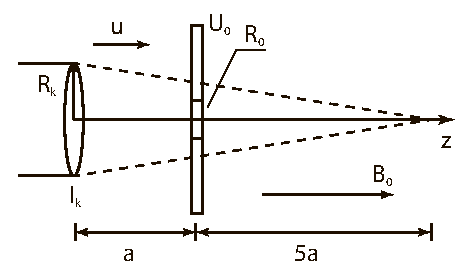
\includegraphics[width=0.5\textwidth]{images/im_03}
    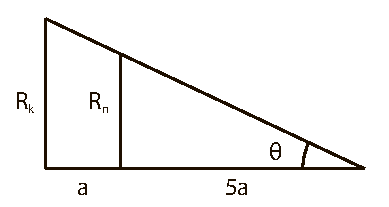
\includegraphics[width=0.5\textwidth]{images/im_04}
\end{wrapfigure}

Найдём радиус отверстия при котором пройдёт весь электронный поток. 
Из рисунка:
\[
	\tan\theta = \frac{R_k}{6a} = \frac{R_\text{п}}{5a} \quad\Rightarrow\quad 
	R_\text{п} \ge \frac{5}{6}R_k
\]

то есть при радиусе отверстия \( 5/6 R_k \) и более весь электронный поток 
пройдёт через диафрагму. 

Рассмотрим движение потока электронов после диафрагмы. Скорость электронов 
\( v_{0z} = u + v_0 \), где \( v_0 \) -- скорость сообщаемая электронам 
диафрагмой. Компонентам электрического потя только \( E_r \) создаваемая 
пространственными зарядами.
\[
	E_r = \frac{\tau}{2\pi\eps_0 r}
\]

где \( \tau \) -- линейная плотность заряда. Выражим её через ток катода и 
скорость электронного потока. 
\[
	\tau = 2\pi r^2 \rho = -\frac{j}{v_{0z}}\cdot 2\pi r^2 = 
	-\frac{I_k}{v_{0z}}
\]
\[
	E_r = - \frac{I_k}{2\pi\eps_0 v_{0z} r}
\]
\[
	\vec{v}\times\vec{B} = \left|\begin{array}{ccc}
		\vec{e}_r & \vec{e}_\phi & \vec{e}_z \\
		\dot{r}   & r\dot{\phi}  & \dot{z}   \\
		B_r       & 0            & B_z
 	\end{array}\right|
\]

Запишем уравнение движения в цилиндрической системе координат:
\[
	\left\{ \begin{array}{ll}
		\ddot{r} - r(\dot{\phi})^2 = -\left|\cfrac{e}{m}\right|
			\left( E_r + B_z r\dot{\phi} \right) \\
		\cfrac{1}{r}\cfrac{d}{dt}(r^2 \dot{\phi}) = 
			-\left|\cfrac{e}{m}\right| 
			\left( B_r \dot{z} - B_z \dot{r} \right)
	\end{array} \right. \eqno{1}
\]

Пусть \( r(z) \) -- траектория электрона в потоке. Вращая данную траекторию 
вокруг оси \( z \) получим поверхность поперечного сечение которой круг 
радиуса \( r \) -- текущая координата крайнего электрона. Рассмотрим поток 
магнитного поля через него.
\[
	\Phi_{(r,z)} = 2\pi \int\limits_{0}^{r} B_z r dr \eqno{2}
\]

Запишем производную потока по времени через частные производные:
\[
	\der{\Phi}{t} = \pder{\Phi}{r}\cdot\der{r}{t} + 
		\pder{\Phi}{z}\cdot\der{z}{t} = 2\pi\left[ B_z r\dot{r} + 
		\dot{r} \int\limits_{0}^{r} \pder{B_z}{z} rdr \right]
\]

Подставляя в неё 
\[
	\div\vec{B} = \frac{1}{r}\pder{}{r}(rB_r) + \pder{B_z}{z} = 0
\]

получаем
\[
	\der{\Phi}{t} = 2\pi r\left[ B_z \dot{r} - \dot{z} B_r \right]
\]

Получаем уравнение левая часть которого совпадает с \( [1.2] \). Подставляя в 
\( [1.2] \) предыдущее уравнение
\[
	\frac{1}{r}\pder{}{t}(r^2\dot{\phi}) = \left|\cfrac{e}{m}\right|
		\frac{1}{2\pi r}\pder{\Phi}{t} \Rightarrow
	\Phi - \Phi_0 = 2\pi\left( r^2 \dot{\phi} - r_0^2 \dot{\phi}_0 \right)
\]

Положим, что начальная плоскость находится в плоскости диафрагмы 
\( \dot{\phi}_0 \) и магнитное поле отсутствует \( \Phi_0 = 0 \), тогда
\[
	\Phi = 2\pi\left|\cfrac{m}{e}\right| r^2 \dot{\phi}
\]

Так как поле имеет только компоненту \( B_z = B_0 \), тогда
\[
	\Phi = 2\pi\int B_0 rdr = \pi r^2 B_0
\]
\[
	\pi r^2 B_0 = 2\pi\left|\cfrac{m}{e}\right| r^2 \dot{\phi} 
		\quad\Rightarrow\quad \dot{\phi} = \frac{1}{2} B_0
		\left|\cfrac{e}{m}\right|
\]

Подставляя полученную \( \dot{\phi} \) в уравнение \( [1.1] \) получаем 
\[
	\ddot{r} - r\left( \frac{1}{2}\left|\frac{e}{m}\right| B_0 \right)^2 = 
		-\left|\frac{e}{m}\right| \left( E_r + \frac{1}{2}B_0^2 r 
		\left|\frac{e}{m}\right| \right)
\]

Преобразуя и подставяя значение для \( E_r \) получим
\[
	\ddot{r} + r\left|\cfrac{e}{m}\right|^2 \frac{B_0^2}{4} - 
		\left|\cfrac{e}{m}\right|\frac{I_k}{2\pi\eps_0 r v_{0z}} = 0
\]

Делая замену вида \( \ddot{r} = v_{0z}^2 \cfrac{d^2 r}{dz^2} \) перейдём к 
уравнению вида:
\[
	\dder{r}{z} + \left|\cfrac{e}{m}\right| \frac{B_0^2}{4v_{0z}^2} r - 
		\left|\cfrac{e}{m}\right| \frac{I_k}{2\pi\eps_0 r v_{0z}^3} = 0
\]

Так как поле \( B(z) = B_0 = const \) и считая, что слева от диафрагмы 
магнитное поле отсутствует. Тогда из предыдущего уравнения следует, что 
при радиуса крайнего электрона 
\[
	r^2_0 = \frac{2I_k}{\pi\eps_0 B^2_0 v_{0z}} \eqno{3}
\]

\( \cfrac{d^2 r}{dz^2} = 0 \) означает отсутствие ускорения по радиусу 
вдоль траектории электрона. Электронный поток, удовлетворяющий условию 
\( [3] \) носит название бриллюэновского потока.

Рассмотрим условие, когда поток незначительно удаляется от равновесного 
радиуса. Введём \( r = r_0 ( 1 + \delta ) \), где \( \delta \ll 1 \) -- 
смещение крайнего электрона в потоке от положения равновесия. Используя 
разложение 
\[ 
	\frac{1}{r} = \frac{1}{r_0(1+\delta)} = \frac{1}{r_0}(1-\delta)
\] 

перейдём к уравнению
\[
	\dder{\delta}{z} + \alpha^2 \delta = 0
\]

где \( \alpha = \left|\cfrac{e}{m}\right|\cfrac{B^2_0}{2v^2_{0z}} \). \\

Решение уравнения можно представить в виде:
\[
	\delta = R_p \cos\left( \alpha z + \beta_0 \right)
\]

где длина волны пульсации потока:
\[
	\alpha = \cfrac{2\pi}{\lambda_p} \quad\Rightarrow\quad
		\lambda_p = \left|\cfrac{m}{e}\right|\cfrac{4\pi v^2_{0z}}{B^2_0}
\] 

Период пульсации 
\[ T_p = \frac{\lambda_p}{c} \]

Радиус пульсации можно найти используя начальные условия:
\[
	R_p = \sqrt{ [\delta(0)]^2 + 
		\left[ \frac{\delta'(0)}{\alpha} \right]^2 }
\]

где \( \delta(0) = \cfrac{R_0}{r_0} - 1 \), 
\( \delta'(0) = \cfrac{r'(0)}{r_0} = -\cfrac{1}{r_0}\tan\theta \)

\begin{figure}[h]
	\begin{minipage}[h]{0.5\linewidth}
		\center{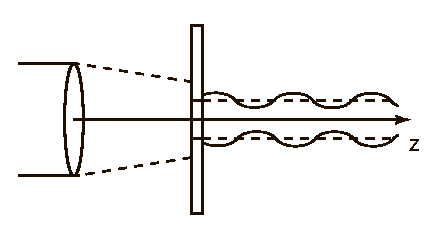
\includegraphics[width=1.0\linewidth]{images/im_05}}
	\end{minipage}
	\begin{minipage}[h]{0.5\linewidth}
		\center{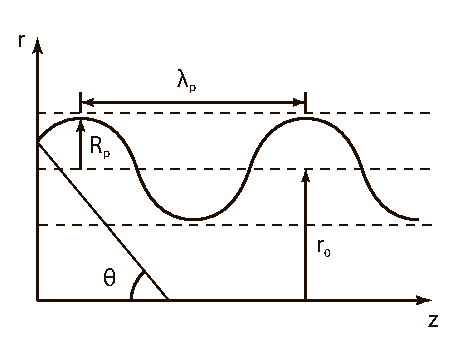
\includegraphics[width=1.0\linewidth]{images/im_06}}
	\end{minipage}
\end{figure}

\end{document}
